% 使用 XeLaTeX 编译；连续编译两次以更新目录与引用。
\documentclass[12pt,a4paper,UTF8]{ctexart}
\usepackage[margin=25mm]{geometry}
\usepackage{graphicx,booktabs,amsmath,amssymb}
\usepackage{enumitem,caption,placeins}
\usepackage[hidelinks]{hyperref}
\graphicspath{{figures/}}
\ctexset{
 section={format=\Large\bfseries\raggedright},
 subsection={format=\large\bfseries\raggedright}
}
\linespread{1.3}
\pagestyle{plain}
\setcounter{tocdepth}{2}
\setlength{\parindent}{0pt}
\setlength{\parskip}{5pt}
\setlength{\emergencystretch}{2em}
\setlist[itemize]{leftmargin=1.5em,itemsep=4pt,topsep=4pt}
\captionsetup{font=small,labelfont=bf}
\renewcommand{\topfraction}{0.9}
\renewcommand{\bottomfraction}{0.8}
\renewcommand{\textfraction}{0.1}
\renewcommand{\floatpagefraction}{0.85}
\newcommand{\ChineseReport}{}
\newcommand{\sectionauthor}[1]{\noindent\textit{章节作者：#1}\par\vspace{3pt}}
\title{\textbf{用电负荷与光伏出力的多步预测}\protect\\[8pt]
\large ELEN90099 深度学习\protect\\Learn--Design--Implement 项目：报告草稿}
\author{Yuchen Yang（学号：1587576）\protect\\Zhengnan Cao（学号：1711701）}
\date{2026 年 10 月}
\begin{document}
\hypersetup{pageanchor=false}
\begin{titlepage}
\maketitle\thispagestyle{empty}
\vfill
\begin{center}\begin{minipage}{0.85\textwidth}
\textbf{草稿状态。} 引言与项目范围已展开；后续章节结合初步发现、简要设计说明和研究计划。Yuchen Yang 负责数据与预处理、实验与分析；Zhengnan Cao 负责模型与理论、引言与结论。
\end{minipage}\end{center}
\end{titlepage}
\pagenumbering{roman}\hypersetup{pageanchor=true}
\tableofcontents\clearpage\pagenumbering{arabic}
% 两位学生的正文目标为 8--10 页，不计封面、目录和参考文献。
% 建议比例：引言 15%，问题定义与范围 35%，实验 35%，结论 15%。

\section{引言}\label{sec:introduction}
\sectionauthor{Zhengnan Cao}
\subsection{项目概述与背景}
用电需求与光伏发电量随时间变化，因此在能源供应和储能安排中，需要对未来一段时间的变化进行预测。与只预测下一个时间点相比，未来一天的完整预测轨迹可以进一步描述需求或出力在何时上升、下降。不过，预测方法也受到可用信息的限制：历史观测可以反映重复出现的规律，却不能直接提供未来天气，也未必包含异常事件发生前的线索。

本项目研究两个独立任务：小时级用电负荷预测与十分钟级光伏出力预测。两者均使用最近 48 小时的数据预测未来 24 小时，每个任务选用固定的 16 个通道，并分别训练模型。Monash 时间序列档案提供了具有不同时间特征的公开预测基准，为这样的对比提供了数据基础\cite{monash}。统一历史长度和预测长度的实际时间跨度，可以在控制项目规模的同时，观察模型在两类能源序列上的表现差异。

项目关注的是：深度学习是否能够在简单日周期重复预测之外带来有用的精度提升，以及这种提升是否值得付出更大的模型和计算成本。当前研究属于监督学习预测，并未实现电力调度或储能控制。本报告展示初步实验与进一步验证计划，预测误差的降低本身不能证明已经获得实际运行收益或经济收益。

\subsection{文献概述与领域研究现状}
选取的文献涵盖几种不同的序列建模思路。LSTM 通过门控记忆保留历史信息，GRU 使用较简化的门控状态\cite{lstm,gru}；时间卷积则通过局部滤波提取变化模式。这些机制为在同一预测任务上比较循环网络、卷积网络及二者组合提供了依据。

相关预测研究也提出了一个值得检验的问题：更复杂的结构是否必然带来更好的结果。Zeng 等人将简单线性模型及分解方法作为复杂预测网络的竞争方案\cite{dlinear}。Nie 等人提出 PatchTST，采用时间块表示和共享权重的通道独立处理\cite{patch}。这两种思路促使本项目同时考察轻量的 DLinear 与时间块注意力模型，但原论文的结论不能直接保证它们在本项目子集和短训练预算下的排名。

草稿中的文献概述围绕实际使用的方法展开。本地注意力模型受到 PatchTST 启发，但并非原论文实现的完整复现。因此，已有论文的基准成绩主要用于说明方法选择的背景，不与本项目的实验分数直接比较。

\subsection{项目范围与任务}
本项目提出三个研究问题。第一，可训练模型是否优于持续性预测和日周期朴素预测？第二，循环、卷积、混合、线性和注意力模型在精度及计算成本上如何取舍？第三，当评价较困难的出力条件，或改变可用历史和训练数据量时，结论是否发生变化？

具体任务包括准备固定数据子集、制定共同评价协议、实现不同模型，以及对比初步结果。输入仅包含历史目标观测，不加入天气预报、日历特征或未来观测。这样的范围有助于明确模型究竟利用了什么信息，也限制了模型对历史中未出现事件的预判能力。报告依照课程要求，从问题定义推进到初步实验，并明确下一阶段工作\cite{course}。

\FloatBarrier
\section{问题定义与范围}\label{sec:problem}
\sectionauthor{Zhengnan Cao：2.1、2.3--2.4 节；Yuchen Yang：2.2 节}
\subsection{问题定义与预测任务}
本项目采用直接多步回归。令 $X\in\mathbb{R}^{T\times C}$ 表示包含 $T$ 个时间点、$C=16$ 个通道的观测序列。在预测起点 $t$，模型读取历史窗口并估计完整的未来目标：
\begin{equation}\label{eq:task}
\widehat{Y}_{t}=f_{\theta}(X_{t-L:t})\in\mathbb{R}^{H\times C},
\qquad Y_t=X_{t:t+H}.
\end{equation}
这里使用左闭右开的切片：输入止于 $t-1$，目标从 $t$ 开始。表~\ref{tab:data} 给出了统一 48 小时历史和 24 小时预测所对应的步数。所有模型均在一次前向计算中输出各通道的全部未来时间点，不将自身的预测递归地作为下一步输入。

\begin{itemize}
\item \textbf{可用信息：} 仅使用预测起点之前已知的观测。不同模型可以联合处理 16 个通道，也可以独立处理各通道并共享权重。
\item \textbf{评价场景：} 测试起点沿时间轴滚动推进，后续起点可以利用新近揭示的观测。因此，这不是在测试区间开始时一次性预测整个测试期。
\item \textbf{预期产出：} 在选定子集上建立可信的模型对比，同时报告原始发布尺度上的误差，以及相对于训练区间季节性参照的误差。
\end{itemize}
共同协议比让所有网络具有相同层数更关键。不同设计使用不同表示和参数规模，这些差异属于模型对比的一部分，也需要在解释结果时加以考虑。

\subsection{相关数据集与预处理}
Electricity Hourly 与 Solar 10 Minutes 文件来自 Monash 所链接的正式发布版本\cite{electricity,solar}。前者包含 321 条小时级序列，后者包含 137 条十分钟级序列。Solar 的源数据包含模拟光伏序列，因此不能将其描述为实地部署观测。每套数据选用 16 个时间对齐的通道；两者属于独立数据集，并非同一个能源系统中的配对观测。

\begin{table}[htbp]
\centering\small\linespread{1.1}\selectfont
\ifdefined\ChineseReport
\caption{数据集与预测任务概况。两个数据集分别建模，均使用 48 小时历史预测未来 24 小时。}
\else
\caption{Datasets and forecasting tasks. Models are fitted separately; both tasks use 48 hours of history to predict the next 24 hours.}
\fi
\label{tab:data}
\begin{tabular}{lrr}
\toprule
\ifdefined\ChineseReport
属性 & Electricity & Solar\\
\midrule
发布序列数 / 选用通道数 & 321 / 16 & 137 / 16\\
每条序列的样本数 & 26,304 & 52,560\\
采样间隔 & 1 小时 & 10 分钟\\
数据年份 & 2012--2014 & 2006\\
历史窗口 $L$（步） & 48 & 288\\
预测时域 $H$（步） & 24 & 144\\
日周期 $m$（步） & 24 & 144\\
训练区间零值占比 & 0.0\% & 53.0\%\\
\else
Property & Electricity & Solar\\
\midrule
Source series / selected channels & 321 / 16 & 137 / 16\\
Samples per series & 26,304 & 52,560\\
Sampling interval & 1 hour & 10 minutes\\
Source years & 2012--2014 & 2006\\
History $L$ (steps) & 48 & 288\\
Horizon $H$ (steps) & 24 & 144\\
Daily period $m$ (steps) & 24 & 144\\
Zero values in training & 0.0\% & 53.0\%\\
\fi
\bottomrule
\end{tabular}
\end{table}


通道名单在所报告的模型对比前固定。选择依据仅使用训练区间的均值：将源序列按平均规模划分为四组，再以种子 42 从每组抽取四条序列。这种方法覆盖了不同的平均量级，未根据测试表现选择通道，但也不足以证明 16 条序列代表了整个数据总体。所选 ID 与数据检查信息均保存在实验记录中。

图~\ref{fig:data} 展示了首个选定通道的前七天观测，以及训练区间的通道相关性。日周期结构支持引入季节性基线。Solar 较高的零值占比也说明需要单独考察活跃出力：整体平均误差较低时，较大出力时段的差异仍可能被掩盖。相关性表明序列具有共同变化，但不能据此断言显式建模通道交互一定能提升预测。

\begin{figure}[htbp]
\centering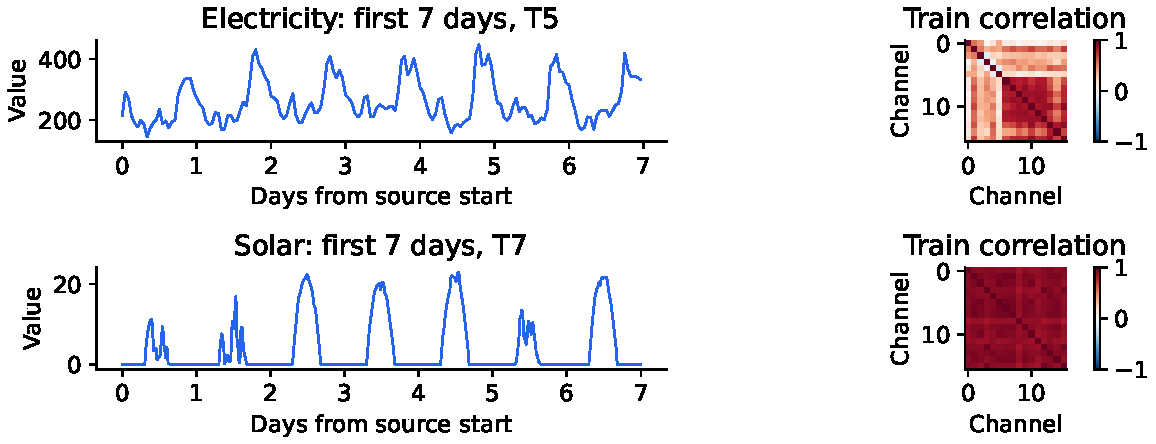
\includegraphics[width=\textwidth,height=7cm,keepaspectratio]{data_overview.pdf}
\caption{固定子集的数据概览：T5 与 T7 的前七天观测，以及仅由训练数据计算的通道相关性。数值保留原始发布尺度。}
\label{fig:data}
\end{figure}

预处理对每个通道分别计算均值和标准差，统计量仅在训练区间拟合。验证集与测试集使用同一组统计量，预测值在评价前转换回原尺度。实验未进行插值或单位换算。现有记录尚未独立确认聚合发布数据的物理单位，因此图表和误差使用原始发布单位。保留源文件的时间网格，不擅自赋予未经确认的当地时区。

\subsection{解决思路与深度学习模型}
实现采用共同预测接口，包含两个无需学习的基线和六个可训练模型。基线在第~\ref{sec:alternatives} 节介绍，深度学习方案概括如下。
\begin{itemize}
\item \textbf{LSTM 与 GRU：} 使用隐藏维度为 64 的单层循环网络，每一步接收全部通道。最终隐藏状态映射到完整的 $H\times C$ 输出；GRU 提供门控结构较简化、循环参数较少的对照。
\item \textbf{1D-CNN：} 两层宽度为三的时间卷积分别使用 32 和 64 个特征通道，配合批归一化和 ReLU，再将时间维自适应平均池化为 16 个位置，连接多步输出头。
\item \textbf{CNN--LSTM：} 宽度为三的卷积先生成 64 维特征，再接 64 单元的 LSTM 和全连接输出头，用于检验局部特征提取能否帮助循环编码。
\item \textbf{DLinear：} 通过 25 步移动平均分离平滑项和剩余项，再用两组线性映射预测未来序列；不同通道共享这些映射。
\item \textbf{PatchTST 风格模型：} 每个通道以长度 16、步长八切分时间块，经 64 维嵌入、两层 Transformer 编码器和线性预测头生成输出；各通道共享权重。
\end{itemize}
注意力实现使用四个头、128 维前馈层、0.1 dropout 和可学习位置编码。它采用训练区间标准化，未实现原模型完整的归一化流程。两种现代模型均为本地编写的具体实现，所以实验对比针对这些设计，不宣称覆盖或复现所有已发表版本。

\subsection{理论基础与方法设计依据}
以下说明各模型的类型、处理历史数据的方式和选择原因，实际效果由实验检验。
\begin{itemize}
\item \textbf{LSTM 和 GRU（循环神经网络）：} 按时间顺序读取数据，用门控保留有用历史，检验记忆是否能帮助预测。但将整个窗口压缩为一个最终状态，也可能丢失信息。
\item \textbf{1D-CNN（一维卷积神经网络）：} 用共享滤波器寻找短时间内的上升或下降，检验局部变化是否有助于预测；学到短期模式不代表也能学到长期规律。
\item \textbf{CNN--LSTM（卷积与循环混合模型）：} 先由 CNN 提取局部特征，再由 LSTM 处理时间顺序，检验两者结合是否有帮助。它也增加了参数，不能把效果变化全部归因于卷积。
\item \textbf{DLinear（分解与线性预测模型）：} 用移动平均得到平滑部分和剩余部分，两者分别经线性映射预测后相加，检验简单结构是否足够有效。剩余部分不一定是日周期变化。
\item \textbf{PatchTST 风格模型（时间块 Transformer）：} 把连续时间点组成块，用注意力寻找有用历史片段，检验分块与逐点处理的差别。各通道独立计算并共享权重，不直接建模通道之间的关系。
\end{itemize}
比较时还要注意采样频率。DLinear 的 25 步移动平均在 Electricity 上覆盖 25 小时，在 Solar 上覆盖 4 小时 10 分钟；PatchTST 风格模型的 16 步时间块分别覆盖 16 小时和 2 小时 40 分钟。因此，即使步数相同，模型看到的实际时间范围也不同，这也可能影响结果。

\FloatBarrier
\section{实验}\label{sec:experiments}
\sectionauthor{Yuchen Yang}
\subsection{实验设置}
每套数据内部的初步实验采用共同协议。以下设置描述已完成的运行；更充分训练与新增控制实验仍属于计划。
\begin{itemize}
\item \textbf{时间划分：} 前 70\% 的观测用于训练，随后 10\% 用于验证，最后 20\% 用于测试。每个完整目标窗口必须落在其所属区间内；输入历史可以延伸到较早区间，因为这些值已经可用。
\item \textbf{预测起点：} 训练窗口每三小时推进一次，验证和测试每小时推进一次。主实验的各模型采用相同起点，Electricity 和 Solar 分别有 5,238 和 1,729 个测试起点。
\item \textbf{训练：} 使用 Adam，学习率 $10^{-3}$、权重衰减 $10^{-4}$、batch size 32、最多五轮、早停耐心三轮。训练损失为标准化 MSE，最终评价使用验证 MSE 最低的权重。
\item \textbf{重复与环境：} 可训练模型的主实验使用种子 42、43、44；实际设备为 NVIDIA GeForce RTX 3060 Laptop GPU，框架为 PyTorch 2.5.1+cu121。这些是本地 GPU 结果，未测量 Colab T4 性能。
\end{itemize}
MAE 衡量平均绝对偏差，RMSE 对较大的误差赋予更高权重。季节性 MASE 将每个通道的 MAE 除以训练区间的平均绝对日周期差，再跨通道平均\cite{mase}；两套数据的日周期分别为 24 步和 144 步。MASE 小于一所参照的是训练尺度，是否优于测试期日周期朴素模型仍需直接检查。两个数据集的原尺度分数不能按数值大小直接比较。

每次运行保存权重、预测、配置和指标，并使用 SQLite 记录实验。已有核验文件记录了 72 次运行的指标复算与权重重载检查。这些检查支持已保存实验的一致性，但不能证明泛化能力。组装本草稿无需新增训练。

\subsection{初步实验结果与验证}
表~\ref{tab:results} 展示主实验对比。可训练模型报告三个种子的均值和样本标准差；持续性预测与日周期朴素预测属于确定性方法，重复记录不产生独立预测试验。这里的标准差描述训练随机性，并不是独立测试日上的置信区间。

% Generated from my_report/submission/report/main_results.csv.
\begin{table}[htbp]
\centering\small\linespread{1.1}\selectfont
\setlength{\tabcolsep}{4pt}
\ifdefined\ChineseReport
\caption{初步测试结果（各数据集每项指标的最低均值加粗）。可训练模型为三个种子的均值 $\pm$ 样本标准差；确定性基线仅列数值。}
\else
\caption{Initial test results; lowest means per dataset and metric are bold. Trainable models: mean $\pm$ SD over three seeds; deterministic baselines: single values.}
\fi
\label{tab:results}
\begin{tabular}{lrrr}
\toprule
Model & MAE & RMSE & MASE\\
\midrule
\multicolumn{4}{l}{\textbf{Electricity}}\\
Persistence & 1,010.261 & 3,091.327 & 3.630\\
Daily naive & 208.218 & 732.211 & 1.009\\
LSTM & 262.727 $\pm$ 4.543 & 727.287 $\pm$ 15.818 & 1.310 $\pm$ 0.015\\
GRU & 262.592 $\pm$ 0.622 & 729.598 $\pm$ 2.779 & 1.304 $\pm$ 0.004\\
1D-CNN & 254.754 $\pm$ 1.493 & 696.794 $\pm$ 17.507 & 1.248 $\pm$ 0.026\\
CNN--LSTM & 267.183 $\pm$ 2.918 & 749.218 $\pm$ 9.099 & 1.310 $\pm$ 0.009\\
DLinear & 220.049 $\pm$ 0.504 & 665.572 $\pm$ 0.484 & 1.032 $\pm$ 0.003\\
PatchTST-style & \textbf{\boldmath 203.137 $\pm$ 3.301} & \textbf{\boldmath 636.246 $\pm$ 6.630} & \textbf{\boldmath 0.959 $\pm$ 0.012}\\
\midrule
\multicolumn{4}{l}{\textbf{Solar}}\\
Persistence & 7.379 & 12.546 & 3.048\\
Daily naive & \textbf{\boldmath 2.198} & 5.712 & \textbf{\boldmath 0.900}\\
LSTM & 3.653 $\pm$ 0.079 & 6.169 $\pm$ 0.192 & 1.493 $\pm$ 0.033\\
GRU & 3.665 $\pm$ 0.131 & 6.126 $\pm$ 0.175 & 1.498 $\pm$ 0.055\\
1D-CNN & 3.020 $\pm$ 0.045 & \textbf{\boldmath 4.888 $\pm$ 0.056} & 1.231 $\pm$ 0.018\\
CNN--LSTM & 3.462 $\pm$ 0.082 & 5.930 $\pm$ 0.146 & 1.414 $\pm$ 0.034\\
DLinear & 3.177 $\pm$ 0.037 & 5.236 $\pm$ 0.017 & 1.298 $\pm$ 0.015\\
PatchTST-style & 3.062 $\pm$ 0.036 & 5.100 $\pm$ 0.058 & 1.249 $\pm$ 0.015\\
\bottomrule
\end{tabular}
\end{table}


Electricity 上，PatchTST 风格模型的 MAE、RMSE、MASE 分别为 203.137、636.246 和 0.959，日周期朴素模型分别为 208.218、732.211 和 1.009。DLinear 的 RMSE 优于日周期朴素模型，但 MAE 和 MASE 更高。因此，单个指标改善不应被描述成预测各方面均改善。

Solar 上，日周期朴素模型具有最低的整体 MAE（2.198）和 MASE（0.900），而 1D-CNN 具有最低的 RMSE（4.888）。这种差异提示方法的误差分布并不相同。五轮训练不足以说明神经网络普遍不适合 Solar；后续需要检验更充分训练后排名是否保持。

\FloatBarrier
\subsection{深度学习模型对比}
初步对比显示，两类任务对应不同取舍：
\begin{itemize}
\item \textbf{Electricity：} 在当前对比中，PatchTST 风格模型的三项整体指标最优。LSTM、GRU 和 CNN--LSTM 未能稳定优于日周期朴素模型。这是关于当前设计及训练预算的证据，不能推广为整个序列模型类别的排名。
\item \textbf{Solar：} 1D-CNN 的整体 RMSE 最低，注意力和分解模型在可训练方案中也具有竞争力。能减少较大偏差的模型，仍可能比保留重复日周期轮廓的基线具有更高的平均绝对误差。
\item \textbf{资源：} Electricity 上 DLinear 有 2,352 个参数，PatchTST 风格模型有 76,056 个。平均训练时间约为 3.0 和 9.4 秒；各运行前向延迟中位数的平均值约为 0.52 和 1.52 ms。它们是本地 GPU 的模型计算结果，不是完整部署延迟。
\end{itemize}
训练时间包含验证过程。延迟测量时输入已经位于设备上，经过十次预热，再进行 30 次同步计时。参数规模和这些时间可以支持初步精度与成本讨论，但不能直接决定嵌入式可行性。容量、算子支持和 Solar 更大的输出头也会影响资源需求。

\subsection{替代方法与基线对比}\label{sec:alternatives}
持续性预测在所有未来时间点重复最后一个观测值。日周期朴素预测则按对应相位重复最近一个完整日周期。二者与神经网络使用相同历史信息，无需拟合参数。由于预测时域恰好为一天，日周期基线不需要输入之外的未来观测。

这两种方法已经完成评价，并非仅为未来建议。两个数据集上的日周期朴素预测均明显强于持续性预测。若 Solar 的首要目标是整体 MAE 或 MASE，日周期朴素方法是当前更有效的选择；在 Electricity 上，它与最佳可训练模型的接近程度也有助于判断增加复杂度是否值得。

预训练时间序列基础模型仅为可选的后续对照，本项目尚未运行此类模型。如果开展扩展，需要保持固定子集、起点和信息限制，并说明预训练是否改变了比较基础。它不属于完成当前终稿实验计划的必要任务。

\subsection{讨论与结果解释}
图~\ref{fig:cases} 按固定规则选取困难样例：使用首个选定通道，寻找包含其最大真实测试目标的最早预测窗口。种子固定为 42，不依据某个模型的误差或最佳种子选图。这些样例可以显示幅值和时序错位，但属于压力情形展示，不能代表全部预测样本。

\begin{figure}[htbp]
\centering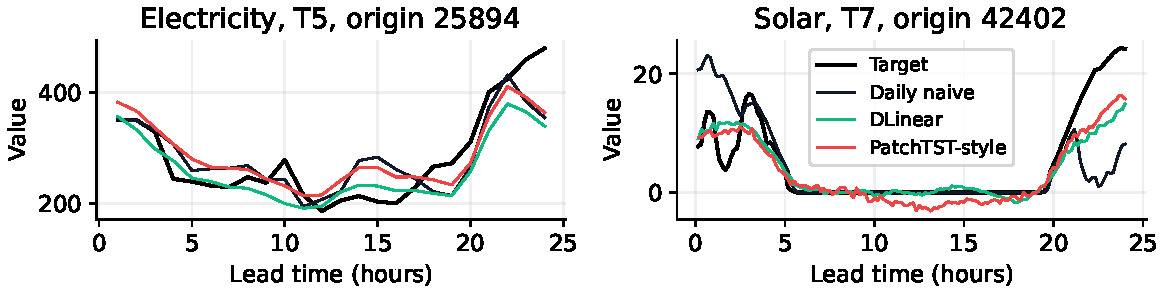
\includegraphics[width=\textwidth,height=6cm,keepaspectratio]{hard_cases.pdf}
\caption{固定规则选择的困难预测样例：Electricity T5（起点 25,894）与 Solar T7（起点 42,402），均使用种子 42。样例依据真实峰值选取，不依据模型预测误差。}
\label{fig:cases}
\end{figure}
\FloatBarrier

\begin{itemize}
\item \textbf{条件误差：} Solar 活跃出力定义为真实值不低于该通道训练最大值的 10\%。PatchTST 风格模型和 DLinear 的活跃出力 MAE 为 4.871、4.896，低于日周期朴素模型的 5.655，但二者整体 MAE 更高。该掩码属于评价条件，不是已验证的日照标签，也不是输入特征。
\item \textbf{已完成的敏感性实验：} LSTM 和 PatchTST 风格模型已测试 24/48/168 小时历史及 25/50/100\% 训练区间，仅使用种子 42。历史对比采用共同起点；结果不支持普遍的单调收益。更长历史也改变注意力模型容量，而数据比例同时影响近期性、季节覆盖和优化更新次数。
\item \textbf{解释边界：} 每小时滚动窗口存在重叠，因此测试误差相互依赖。现有测试区间在项目开发中已经查看，不能称为完全未触碰的外部盲测，也不据此作独立窗口显著性结论。
\end{itemize}
主分数保留未经裁剪的负预测。统一非负裁剪可以作为单独的后处理对照研究。更完整的预测距离和通道误差分析留到终稿，重点检查改善是否发生在对当前任务有意义的条件下。

\FloatBarrier
\section{结论}\label{sec:conclusion}
\sectionauthor{Zhengnan Cao}
\subsection{项目反思与综合讨论}
初步研究的主要认识是：有用的模型对比应从明确任务和强基线开始。在固定 Electricity 子集上，当前时间块注意力设计相对于日周期朴素模型改善了三项整体误差。Solar 上，日周期重复仍具有更低的整体 MAE 和 MASE，而卷积及其他可训练模型在不同指标或出力条件下表现出优势。因此，初始问题的答案依赖具体任务及评价目标。

实验也提示应区分结构机制与测量结果。门控、局部滤波、分解和时间块注意力都为时间信息表示提供了合理思路，但当前实验没有隔离这些机制的独立影响。网络容量和表示不同，五轮训练也不保证各模型达到可比的收敛程度。所以，这些结果支持继续研究具体方案，而非普遍推荐某一个模型。

现有证据局限于每个数据集的 16 个通道和一个时序测试区间。Solar 的模拟来源以及缺少天气信息，进一步限制了对真实光伏运行的推论。资源结果只描述一台本地笔记本 GPU 上的模型计算；无论精度还是时间测量，都不能证明已经实现经济收益、储能控制收益或部署就绪。

本草稿的阶段贡献在于共同协议、可运行的模型实现、初步对比，以及可以继续检验的问题。数据流程与已保存记录为这些检验提供了基础。终稿应进一步说明哪些发现能在更充分控制的实验中保持，哪些初始解释需要修正。

\subsection{后续研究方向}
下一阶段工作直接对应上述局限。以下内容属于计划任务，尚未作为完成结果报告。
\begin{itemize}
\item \textbf{更充分训练：} 检查训练和验证曲线，将训练上限扩展到 20 轮，并在相近调参预算下进行小规模、明确记录的验证集搜索。保持固定子集和评价起点，不按测试分数选择偏好的种子。
\item \textbf{重复敏感性研究：} 对现有历史长度和数据比例设置进行多种子重复，同时报告 MAE、RMSE 和 MASE。增加优化更新次数匹配对照，区分数据可用量与训练投入的影响。
\item \textbf{容量匹配消融：} 对比 CNN--LSTM 与考虑参数规模的循环控制模型，测试移除卷积前端，以判断前端的价值是否超出增加容量本身。
\item \textbf{进一步误差分析：} 分析不同通道和预测距离，增加预先定义的困难情形，对比统一非负裁剪。若估计统计不确定性，应采用尊重重叠窗口依赖的时间块方法。
\end{itemize}
完成标准是更清楚地解释共同协议下的模型行为，而不是要求最复杂的结构必须胜出。尚未完成的任务将明确列出，最终结论也将限定在实际数据和验证证据能够支持的范围内。

\label{report:body-end}
\clearpage\phantomsection\addcontentsline{toc}{section}{参考文献}
% Shared numbered bibliography; original records checked on 14 October 2026.
\begin{thebibliography}{9}
\small
\bibitem{monash} R. Godahewa, C. Bergmeir, G. I. Webb, R. J. Hyndman, and P. Montero-Manso, \emph{Monash Time Series Forecasting Archive}, NeurIPS Datasets and Benchmarks, 2021. \url{https://arxiv.org/abs/2105.06643}.
\bibitem{lstm} S. Hochreiter and J. Schmidhuber, \emph{Long Short-Term Memory}, Neural Computation, vol. 9, no. 8, pp. 1735--1780, 1997. \url{https://www.bioinf.jku.at/publications/older/2604.pdf}.
\bibitem{gru} K. Cho et al., \emph{Learning Phrase Representations using RNN Encoder-Decoder for Statistical Machine Translation}, EMNLP, pp. 1724--1734, 2014. \url{https://arxiv.org/abs/1406.1078}.
\bibitem{dlinear} A. Zeng, M. Chen, L. Zhang, and Q. Xu, \emph{Are Transformers Effective for Time Series Forecasting?} AAAI, vol. 37, no. 9, pp. 11121--11128, 2023. \url{https://doi.org/10.1609/aaai.v37i9.26317}.
\bibitem{patch} Y. Nie, N. H. Nguyen, P. Sinthong, and J. Kalagnanam, \emph{A Time Series is Worth 64 Words: Long-term Forecasting with Transformers}, ICLR, 2023. \url{https://arxiv.org/abs/2211.14730}.
\bibitem{electricity} R. Godahewa et al., \emph{Electricity Hourly Dataset}, version 3, Zenodo, 2020. \url{https://doi.org/10.5281/zenodo.4656140}.
\bibitem{solar} R. Godahewa et al., \emph{Solar Dataset (10 Minutes Observations)}, version 3, Zenodo, 2020. \url{https://doi.org/10.5281/zenodo.4656144}.
\bibitem{mase} R. J. Hyndman and A. B. Koehler, \emph{Another Look at Measures of Forecast Accuracy}, International Journal of Forecasting, vol. 22, no. 4, pp. 679--688, 2006. \url{https://doi.org/10.1016/j.ijforecast.2006.03.001}.
\bibitem{course} ELEN90099 teaching team, \emph{LDI Project Manual v1 and Prelim Report Instructions}, University of Melbourne, 2026. Supplied course materials.
\end{thebibliography}

\end{document}
